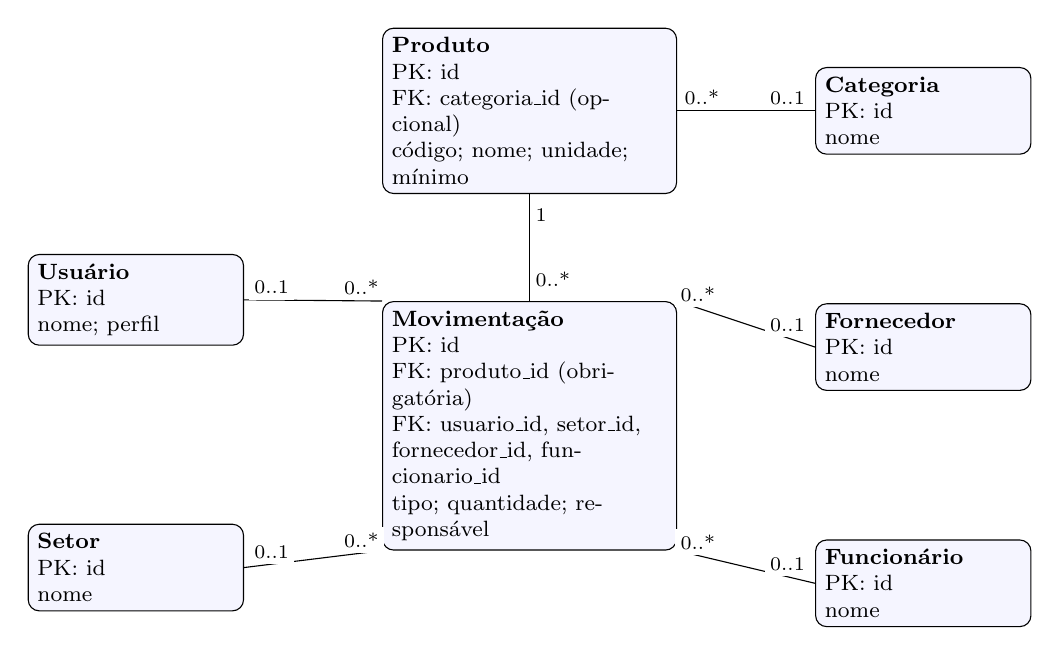
\begin{tikzpicture}[every node/.style={font=\footnotesize}, entity/.style={draw,rounded corners,align=left,text width=2.5cm,minimum height=1.1cm,fill=blue!4},card/.style={font=\scriptsize,fill=white,inner sep=2pt}]
\node[entity,text width=3.5cm] (mov) at (0,0) {\textbf{Movimentação}\\PK: id\\FK: produto\_id (obrigatória)\\FK: usuario\_id, setor\_id,\\fornecedor\_id, funcionario\_id\\tipo; quantidade; responsável};
\node[entity,text width=3.5cm] (prod) at (0,4) {\textbf{Produto}\\PK: id\\FK: categoria\_id (opcional)\\código; nome; unidade; mínimo};
\node[entity] (cat) at (5,4) {\textbf{Categoria}\\PK: id\\nome};
\node[entity] (usr) at (-5,1.6) {\textbf{Usuário}\\PK: id\\nome; perfil};
\node[entity] (set) at (-5,-1.8) {\textbf{Setor}\\PK: id\\nome};
\node[entity] (forn) at (5,1) {\textbf{Fornecedor}\\PK: id\\nome};
\node[entity] (func) at (5,-2) {\textbf{Funcionário}\\PK: id\\nome};
\draw (mov.north) -- node[card,pos=0.2,right] {0..*} node[card,pos=0.8,right] {1} (prod.south);
\draw (prod.east) -- node[card,pos=0.18,above] {0..*} node[card,pos=0.8,above] {0..1} (cat.west);
\draw (mov.north west) -- node[card,pos=0.15,above] {0..*} node[card,pos=0.8,above] {0..1} (usr.east);
\draw (mov.south west) -- node[card,pos=0.15,above] {0..*} node[card,pos=0.8,above] {0..1} (set.east);
\draw (mov.north east) -- node[card,pos=0.15,above] {0..*} node[card,pos=0.8,above] {0..1} (forn.west);
\draw (mov.south east) -- node[card,pos=0.15,above] {0..*} node[card,pos=0.8,above] {0..1} (func.west);
\end{tikzpicture}
